% Options for packages loaded elsewhere
\PassOptionsToPackage{unicode}{hyperref}
\PassOptionsToPackage{hyphens}{url}
%
\documentclass[
]{article}
\title{Adaptive Conformal Inference}
\author{Drew Keller, Charles Mayville}
\date{3/8/2023}

\usepackage{amsmath,amssymb}
\usepackage{lmodern}
\usepackage{iftex}
\ifPDFTeX
  \usepackage[T1]{fontenc}
  \usepackage[utf8]{inputenc}
  \usepackage{textcomp} % provide euro and other symbols
\else % if luatex or xetex
  \usepackage{unicode-math}
  \defaultfontfeatures{Scale=MatchLowercase}
  \defaultfontfeatures[\rmfamily]{Ligatures=TeX,Scale=1}
\fi
% Use upquote if available, for straight quotes in verbatim environments
\IfFileExists{upquote.sty}{\usepackage{upquote}}{}
\IfFileExists{microtype.sty}{% use microtype if available
  \usepackage[]{microtype}
  \UseMicrotypeSet[protrusion]{basicmath} % disable protrusion for tt fonts
}{}
\makeatletter
\@ifundefined{KOMAClassName}{% if non-KOMA class
  \IfFileExists{parskip.sty}{%
    \usepackage{parskip}
  }{% else
    \setlength{\parindent}{0pt}
    \setlength{\parskip}{6pt plus 2pt minus 1pt}}
}{% if KOMA class
  \KOMAoptions{parskip=half}}
\makeatother
\usepackage{xcolor}
\IfFileExists{xurl.sty}{\usepackage{xurl}}{} % add URL line breaks if available
\IfFileExists{bookmark.sty}{\usepackage{bookmark}}{\usepackage{hyperref}}
\hypersetup{
  pdftitle={Adaptive Conformal Inference},
  pdfauthor={Drew Keller, Charles Mayville},
  hidelinks,
  pdfcreator={LaTeX via pandoc}}
\urlstyle{same} % disable monospaced font for URLs
\usepackage[margin=1in]{geometry}
\usepackage{graphicx}
\makeatletter
\def\maxwidth{\ifdim\Gin@nat@width>\linewidth\linewidth\else\Gin@nat@width\fi}
\def\maxheight{\ifdim\Gin@nat@height>\textheight\textheight\else\Gin@nat@height\fi}
\makeatother
% Scale images if necessary, so that they will not overflow the page
% margins by default, and it is still possible to overwrite the defaults
% using explicit options in \includegraphics[width, height, ...]{}
\setkeys{Gin}{width=\maxwidth,height=\maxheight,keepaspectratio}
% Set default figure placement to htbp
\makeatletter
\def\fps@figure{htbp}
\makeatother
\setlength{\emergencystretch}{3em} % prevent overfull lines
\providecommand{\tightlist}{%
  \setlength{\itemsep}{0pt}\setlength{\parskip}{0pt}}
\setcounter{secnumdepth}{-\maxdimen} % remove section numbering
\usepackage{mathtools}
\ifLuaTeX
  \usepackage{selnolig}  % disable illegal ligatures
\fi

\begin{document}
\maketitle

\hypertarget{summary}{%
\section{Summary}\label{summary}}

With the increased prevalence of less-interpretable models like machine
learning algorithms, the importance of distribution-free tools quantify
the prediction uncertainty rises (especially since these classes of
models are less explicit in what drives their predictions and where they
might go wrong).

One of the most popular approaches to address this problem is conformal
inference. Conformal inference allows us to measure the predictive power
of otherwise non-transparent models by calculating a ``conformity
score'' on model generated predictions and their observed counterparts.
However, conformal inference relies quite heavily on exchangeability
assumptions, which are often not met in real world applications, in
particular settings that are heavily time dependent.

In response, Gibbs and Candès (I. Gibbs and E. Cand`es, ``Adaptive
conformal inference under distribution shift,'' arXiv:2106.00170, 2021.)
devise a new method: adaptive conformal inference (ACI). ACI works to
measure predictive power of models in settings without exchangeability
in which data is revealed incrementally, by adjusting the procedure
based on the coverage rate in each time step.

They show that given a long enough time, ACI meets target coverage
without additional assumptions in situations where standard conformal
inference fails. Additionally they show that given small distribution
assumptions, ACI is robust for most time steps.

The authors test their new procedure on two datasets, election
predictions and stock price predictors. In both cases they confirm their
theoretical results, ACI maintained approximately 90\% coverage while
conformal inference failed, often dramatically.

We seek to extend ACI for use on batch data, and test empirically the
effects of allowing varying quantile and score functions.

\hypertarget{intuitive-explanation}{%
\subsection{Intuitive Explanation}\label{intuitive-explanation}}

The goal of conformal inference is to produce a confidence interval for
a new prediction. (The authors' equivalent formulation: determine if
some value y is a ``reasonable'' estimate.) In essence, we are looking
at where some percentage of the most ``unusual'' predictions have fallen
so far, and stating that outside of that interval, the same percentage
of future predictions should be similarly unusual. The split conformal
inference process is to: (a) fit some ``conformity score'' on a subset
of the data (``training set'') that characterizes how well each model
prediction matches the corresponding actual value, (b) calculate
conformity scores on the rest of the data (``holdout'' or ``calibration
set''), (c) find the \((1-\alpha)^{th}\) quantile of the calibration
conformity scores, and (d) infer the prediction interval as the range in
which \(S(X_{t+1},y)\le \hat Q (1-\alpha)\).

When new data points are generated from the same process, our quantile
will still contain each new point's conformity score with the same
probability. However, if new data points are generated from a different
process -- a distribution shift -- then their conformity scores may be
more or less likely to fall within our quantile. This paper suggests
that we can account for this fact and maintain the same probability of
coverage in the long term by updating our quantile cutoff based on
whether or not we cover each new prediction.

The paper suggests making this update by decreasing our quantile by
\(\gamma\alpha\) if we covered the last prediction or increasing it by
\(\gamma(1-\alpha)\) if we do not, using some heuristically- or
empirically-selected step size \(\gamma\). Note that for low alpha, we
increase our quantile cutoff much more quickly when we fail to cover
than we decrease it when we do cover (for example, for
\(\alpha = 0.05\), \(\gamma(1-0.05) = 0.95\gamma >> \gamma(0.05)\)).
This makes sense because, with correct \(\alpha=0.05\) coverage, we
expect to cover 95\% of the time and miss 5\% of the time -- so our
adjustments in each direction should be weighted to reflect that a miss
is more ``surprising'' than a cover.

This ``adaptive conformal inference'' procedure allows us to ensure that
in the long run, we will achieve our targeted coverage frequency. Even
in the short run, the local coverage rate will stay relatively close to
the target as long as the distribution doesn't shift too drastically.

\hypertarget{main-theoretical-results}{%
\section{Main Theoretical Results}\label{main-theoretical-results}}

The authors define their adaptive conformal inference procedure as an
online update to the quantile cutoff in the setting in which the true
value \(Y_t\) is revealed after each prediction \(y\). Specifically, the
authors point out that there is a value \(\alpha^*_t\) such that the
miscoverage rate of the prediction set up to \(t\) is \(\alpha\) when we
use \(1-\alpha^*_t\) as our quantile cutoff. The authors propose the
following procedure to estimate \(\alpha^*_t\) at each time step (with
the estimate called \(\alpha_t\), initialized to \(\alpha\) in their
experiments):

\[ \textrm{err}_t := 
\left \{
\begin{array}{ll}
1 & \textrm{if } Y_t \notin \hat{C}_t(\alpha_t), \\
0 & \textrm{otherwise} \\
\end{array} 
\right. 
\] where
\[ \hat{C}_t (\alpha_t) := {y : S_t(X_t, y) \le \hat{Q}_t(1 - alpha_t)} \]
Then, fixing a step size parameter \(\gamma > 0\) we consider the simple
online update
\[ \alpha_{t+1} := \alpha_t + \gamma(\alpha - \textrm{err}_t). \]

Substituting \(\textrm{err}_t\) into \(1-\alpha_{t+1}\), this procedure
sets the \(t+1\) quantile cutoff as:
\(1-\alpha_{t+1} = 1- (\alpha_t + \gamma(\alpha-1)) = 1 - \alpha_t + \gamma(1-\alpha)\)
when we fail to cover and
\(1-\alpha_{t+1} = 1- (\alpha_t + \gamma(\alpha-0)) = 1 - \alpha_t - \gamma\alpha\)
when we do cover.

A higher step size \(\gamma\) makes the method more adaptive to
distribution shifts but also can make local coverage more variable;
lower \(\gamma\) makes the method less adaptive (\(\gamma=0\) is
equivalent to standard split conformal inference) but moves more towards
conditional coverage with respect to time. The authors do not propose a
theory-based means of selecting \(\gamma\) (they do note that the
optimal alpha is proportional to the square root of a quantification of
distribution shift, but this is unobserved so is unhelpful in practice).
However, they say that \(\gamma=0.005\) empirically worked well with
their datasets.

The authors also note that the procedure can be easily modified to give
some weight to previous coverage/noncoverage events in updating
\(\alpha_t\), essentially adding some momentum to the update.
Specifically:

\[ \alpha_{t + 1} = \alpha_t + \gamma(\alpha - \sum_{s=1}^t w_s \textrm{err}_s) \]

where weights are \(\in[0,1]\) and sum to 1. (Obviously, \(w_t=1\) is
equivalent to the unweighted method.) However, the authors say that
though weighting may somewhat smooth local coverage, in their
experiments it produces similar results to unweighted updates.

The authors note that this adaptive inference procedure works for any
choice of quantile and score functions (assuming those functions are
definitionally valid, e.g.~the quantile function must be nondecreasing).
However, they also acknowledge that the procedure's performance is
sensitive to quality of conformity scores. In particular, the closer to
stationary the conformity score (despite shifts in the data
distribution), the closer the procedure will stay to target coverage.

The authors do not spend much time addressing the choice of initial
\(\alpha_0\), but it seems clear that \(\alpha_0=\alpha\) should be the
best choice in the absence of any prior beliefs about the magnitude and
direction of distribution shift.

The authors prove two main performance guarantees for the procedure.
First, they show that over a long time interval, adaptive conformal
inference converges on the targeted coverage frequency without any
distributional assumptions:

\[ \lim_{T \to \infty} \frac{1}{T} \sum_{t=1}^T \textrm{err}_t \stackrel{a.s.}{=} \alpha.\]

Then, they show that for a sufficiently small distribution shift (and
appropriate initialization of \(\alpha_1\)), the marginal coverage rate
will stay close to 1-\(\alpha\) in expectation. Specifically, the
authors prove this result in the case in which the data originates from
distributions associated with the states of a hidden Markov chain with a
stationary distribution. The authors acknowledge that this model may not
directly apply to the real world, but argue that the results are a good
approximation of the procedure's behavior in many real-world settings.

(To analyze this claim a bit: Two cases in which this model would not be
applicable are when the data distribution shifts seasonally or with a
continual trend, as the corresponding Markov process would be periodic
or contain infinite transient states, respectively, and so would have no
stationary distribution. But note that these cases are where the data
distribution has a trend or is seasonal; trend or seasonality in \(X\)
and \(y\) is fine as long as their joint distribution remains the same.
Also, predictable distribution shift could be handled in the long run by
adding a time variable to \(X\). A more problematic case is that of the
infinite null recurrent Markov chain, eg a number line random walk.)

This second performance guarantee also requires a few other assumptions:
that an initialization period has passed such that the Markov process
has reached its stationary distribution, and that the quantile and score
functions are fixed in time. The latter assumption is potentially rather
limiting as this is not how the procedure would typically be
implemented; in practice we would want to retrain the functions as we
get additional data.

The actual result shown by the authors is the following:

\[ E[(M(\alpha_t | A_t) - \alpha)^2 ] \le \frac{L(1 + \gamma)}{\gamma} E [ | \alpha_{A_{t+1}}^* -\alpha_{A_t}^* | ] + \frac{L}{2} \gamma \]

where \(M\) is the realized miscoverage rate, \(A\) indicates the hidden
state of the underlying Markov model, and \(L\) is a positive constant
such that
\[ | M(\alpha_2 | a) - M(\alpha_1 | b) | \le L | \alpha_2 - \alpha_1 | \]
for any \(\alpha_1,\alpha_2\) and any Markov state \(a\) in the chain.
(The authors also prove an intermediate result showing that the
miscoverage rate's distance from \(\alpha\) is bounded over sufficiently
long time periods.) The left-hand side of the inequality result is the
expected Euclidean distance between marginal misclassification rate and
\(\alpha\). Since \(\gamma\) is typically small, the right-hand-side of
the inequality will be small, bounding the misclassification rate near
\(\alpha\). The right-hand-side expectation quantifies the distribution
shift, showing that the distance between marginal coverage and alpha is
bounded more tightly when the distribution shift is small.

\hypertarget{limitations}{%
\section{Limitations}\label{limitations}}

Gibbs and Candès point out three limitations with their method. First,
their method is devised with the assumption that data is revealed in an
online manner: the true value of each time step is revealed before
prediction of the next time step. While this assumption is met in some
cases (like stock market data), there are many settings in which data is
received in batches. On top of making it hard to evaluate settings where
data is irregular over time, it prevents the evaluation scheme from
distinguishing between ``bad'' prediction subsets and ``good'' ones
merely by conditioning on time.

Another limitation of the more strict theoretical performance result is
that the authors assume a fixed quantile function, \(\hat{Q}(\cdot)\),
predetermined without influence from new data. Gibbs and Candès prove
that fitting \(\hat{Q}_t(\cdot)\) in an online fashion to the most
recent data similar to \(\alpha_t\) will provide correct coverage given
sufficiently large time intervals. However, the proof of short term
bounds given good initialization of \(\alpha_1\) relies on a fixed
\(\hat{Q}(\cdot)\), limiting the theoretical performance of the fully
online method. The online method was used in their following
experiments, showing that it does have practical success. We further
investigate this discrepancy below.

A third limitation of the procedure is that the authors specify no
theoretical guidelines for choosing an effective \(\gamma\). A proper
choice of step size for the data is extremely important, as too large
values of \(\gamma\) induce volatility in the coverage produced at each
step \(\alpha_t\). In their experiments they settle on a choice of
\(\gamma = 0.005\), but acknowledge that this has no guarantee of
success in other applications.

A limitation not mentioned by the authors comes from common procedures
to reduce the computational complexity of conformal inference methods.
One such procedure is to limit the calculation of the prediction set to
the interval observed in the data. In standard conformal inference, this
simplification is guaranteed to not adjust the coverage by much for
large \(n\), as:

\[ \hat{C}'(X_{n+1}) = \hat{C}(X_{n+1}) \cap \textrm{range}_{ 1 \le i \le n} (Y_i) \]
\[ P(Y_{n+1} \in \hat{C}'(X_{n+1}) ) \ge P(Y_{n+1} \in \hat{C}'(X_{n+1}) - P(Y_{n+1} \notin \textrm{range}_{ 1 \le i \le n} (Y_i)  \ge 1 - \alpha - \frac{2}{n + 1} \textrm{ by exchangeability } \]

But since

\begin{enumerate}
\def\labelenumi{\arabic{enumi}.}
\tightlist
\item
  ACI does not assume exchangeability for all \((Y_1, … , Y_{n+1})\),
  and
\item
  ACI calculates \(\hat{C}_t (\cdot)\) in an online fashion, making the
  bound dependent on time even if exchangeability was met
\end{enumerate}

ACI may not be able to make a similar time saving procedure, hampering
practical performance unless some assumptions are conceded.

\hypertarget{extension-batched-procedure}{%
\section{Extension: Batched
Procedure}\label{extension-batched-procedure}}

As pointed out previously, one limitation of the procedure is that it is
unable to handle data received in delayed batches, and may mistreat data
in cases without data collectable on uniform time increments.

An intuitive extension to ACI that may work better in these cases is a
procedure that updates \(\alpha\) based on coverage rate in chunks
(either defined by intervals of discrete time or regularly spaced
batches of data). Consider the following procedure:

Given data \((X_{s_i}, Y_{s_i})\) in discrete chunks enumerated
\((X_s, Y_s)\). Assume for each data point \(s_i\) we are given a fitted
score function \(S_{s_i}(\cdot)\) and a corresponding quantile function
\(\hat{Q}_{s_i}(\cdot)\). Then, in similar fashion to the old procedure
define the realized miscoverage rate of the prediction set
\(\hat{C}_{s_i}(\alpha_s) := \{ y : S_{s_i}(X_{s_i}, y) \le \hat{Q}_{s_i}(1-\alpha_s) \}\)
as

\[ M_s(\alpha_s) := P(S_s(X_s, Y_s) > \hat{Q}_s(1-\alpha_s)). \]

Define the sequence \(\alpha_s\) given a target \(\alpha\), fixing a
step size parameters \(\gamma > 0\) as:

\[ \alpha_{s+1} := \alpha_s + \gamma(\alpha - \textrm{err}_s). \] for
\(\textrm{err}_s\):
\[ \textrm{err}_s := \frac{1}{\textrm{# i in s}}\sum_{i \in s}
\mathbb{1} \{ Y_{s_i} \notin \hat{C}_{s_i}(\alpha_s)\}
\]

Intuitively what we are doing is rather than adjusting the value of
\(\alpha\) for every data point \(s_i\), we are adjusting it per chunk
of data \(s\) by the rate of coverage in that chunk.

An important note here regards the choice of \(\gamma\) for this
procedure. A good rule of thumb is to select \(\gamma\) that is higher
than the \(\gamma\) used in the original method by roughly a factor of
the number of data points per time step, or slightly below. (Or, we
could define the procedure such that each adjustment is proportional to
the number of time steps in the relevant batch, which would be
preferable for variable batch sizes but reduce flexibility for
constant-size batches.) Otherwise, this procedure will adjust
\(alpha_t\) too slowly relative to the original procedure. The reason
that we might select \(\gamma\) slightly lower than a simple multiple of
original \(\gamma\) is that using the simple multiple, the batched
procedure will adjust \(\alpha_t\) by \emph{more} than the online
procedure, since the online procedure's updates will reduce as
\(\alpha_t\) approaches \(\alpha_t^*\).

A final note here: In the alternative setting in which we receive
batches of data in which we \emph{do} know the ordering of data in the
batch, it is likely preferable to use the original online procedure in
order to not ``overshoot'' \(\alpha_t^*\) (though the online procedure
is somewhat more computationally expensive).

\hypertarget{long-term-coverage-for-modified-procedure}{%
\subsection{Long term coverage for modified
procedure}\label{long-term-coverage-for-modified-procedure}}

Following similar steps to the proof outlined for the standard ACI, we
can get some long term coverage guarantee for our modified procedure. We
will similarly assume that with probability one \(\alpha_1 \in [0, 1]\)
and \(\hat{Q}_{s_i}(\cdot)\) is non decreasing and is \(\infty\) for
inputs greater than one and \(-\infty\) for inputs less than zero.

\textbf{Lemma 4.1 adjusted}: with probability one we have that
\(\forall s \in \mathbb{N}, \alpha_s \in [-\gamma, 1+\gamma]\).

\emph{Proof}: assume towards a contradiction that with positive
probability \(\{\alpha_s\}_{s \in \mathbb{N}}\) is such that
\(\inf_s \alpha_s < -\gamma\) (the case where
\(\inf_s \alpha_s > 1 + \gamma\) is identical). Note that
\(\sup_s |\alpha_{s+1} − \alpha_s| = \sup_s \gamma | \alpha − \textrm{err}_s| < \gamma\).
Thus, with positive probability we may find \(s \in \mathbb{N}\) such
that \(\alpha_s < 0\) and \(\alpha_{s + 1} < \alpha_s\). However,

\[ \alpha_s < 0 \implies \hat{Q}_{s_i} (1 - \alpha_s) \forall i \in s \implies \textrm{err}_s = 0 \implies \alpha_{s+1} = \alpha_s + \gamma(\alpha - \textrm{err}_s) \ge \alpha_s \]

and thus
\(P(\exists s \textrm{ such that } \alpha_{s+1} < \alpha_s < 0) = 0\),
which is a contradiction.

\textbf{Proposition 4.1 adjusted}: with probability one we have that
\(\forall S \in \mathbb{N}\),

\[ | \frac{1}{S} \sum_{s=1}^S \textrm{err}_s - \alpha | \le \frac{\max \{ \alpha_1, 1- \alpha_1 \} + \gamma}{S \gamma} \]

which implies

\[ \lim_{S \to \infty} \frac{1}{S} \sum_{s=1}^S \textrm{err}_s \stackrel{a.s.}{=} \alpha \]

\emph{Proof}: expanding the recursion for \(\alpha_s\) and applying
lemma 4.1 adjusted in the same way as for the original method yields the
result, since the recursion for \(\alpha_s\) and \(\alpha_t\) share the
same structure.

Thus our modified procedure has a similar agnostic guarantee of correct
long-term coverage frequency as standard ACI.

\hypertarget{modified-procedure-in-practice}{%
\subsection{Modified procedure in
practice}\label{modified-procedure-in-practice}}

To get a quick comparison between the standard method and the modified
one we ran the modified procedure on the same data set as those run for
the standard procedure (NVIDIA and Fannie Mae stock data), with a target
coverage level of 90\%. To do this, we simply grouped the otherwise
perfectly distributed data into specified chunk sizes for our two runs
of the modified procedure. For some details on the author's code, see
the caveat in the next section.

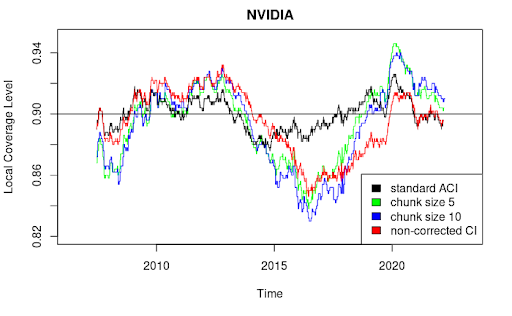
\includegraphics[width=0.5\textwidth,height=\textheight]{./images/1nvidiamodified.png}
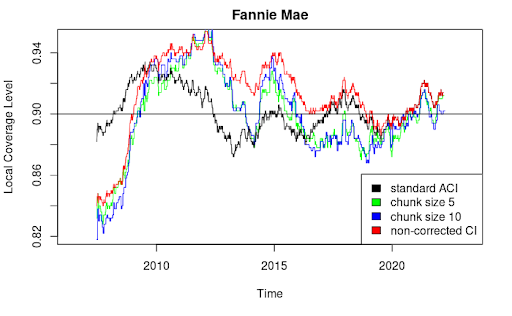
\includegraphics[width=0.5\textwidth,height=\textheight]{./images/2fmmodified.png}

We do see less robustness with changes to time than standard ACI, but
this is to be expected, as we have less effective time to converge to
good values of alpha, and less points in time to adjust to shifts in the
underlying distribution, however the effect is too large for this to be
the only cause. A possible cause for this effect is that in taking large
batches of data, we are effectively increasing the pressure that our
small choice of \(\gamma\) has on the data. If the modified and standard
ACI procedures choose the same \(\gamma\), in the time interval of the
batch the standard procedure will update with \(\gamma\) many times,
where as the modified procedure will only update once.

If we correct our choice of \(\gamma\) to be scaled by the time size of
the batch, we get results that are similarly robust to changes in time
as standard ACI, confirming our hypothesis.

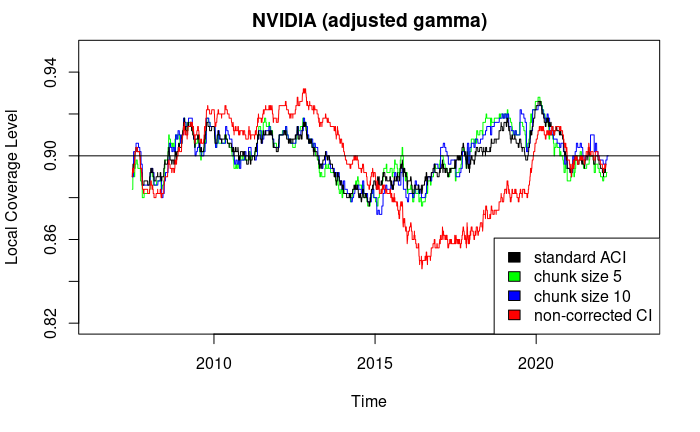
\includegraphics[width=0.5\textwidth,height=\textheight]{./images/9nvidiamodifiedadj.png}
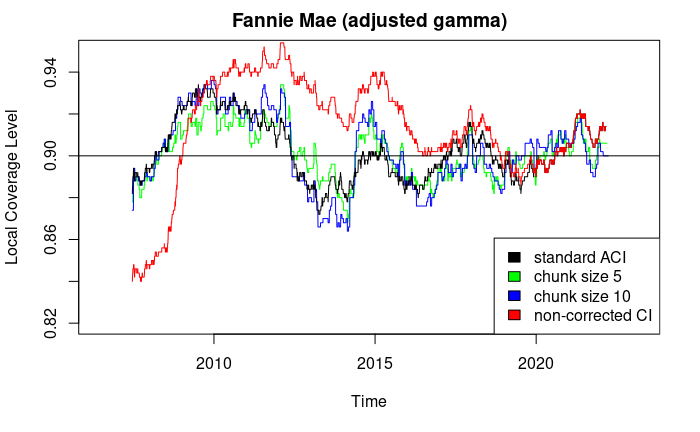
\includegraphics[width=0.5\textwidth,height=\textheight]{./images/10fmmodifiedadj.png}

This reinforces how important appropriate \(\gamma\) selection is
practice of both the modified and standard methods.

\hypertarget{experiment-how-applicable-is-the-fixed-qs-setting}{%
\section{Experiment: How Applicable is the Fixed-QS
Setting?}\label{experiment-how-applicable-is-the-fixed-qs-setting}}

Intuitively, we might expect varying-\(QS\) to perform better than
fixed-\(QS\) in a distribution-shifting setting, both because this
provides a larger amount of training/calibration data and because it
essentially adjusts \(S\) and \(Q\) in addition to \(\alpha_t\) in
response to distribution shift. On the other hand, it is possible that
the approach used by the authors in their experiments -- refitting \(S\)
and \(Q\) on the previous \texttt{lookback} data points at each time
step (they use \texttt{lookback=1250} in their stock analysis) -- is
subject to overfitting issues due to the reuse of the same data for
score training and quantile calibration.

As the authors allude to, it's difficult to obtain analytical results
for varying-\(QS\) performance. So, we used the same stock-volatility
example as the authors to explore the differences in results between
fixed-\(QS\) and varying-\(QS\) approaches.

Specifically, we replicate the authors' experimental results shown in
Figure 1 for NVIDIA and Fannie Mae, then repeat the same analysis but
using \(S(\cdot)\) trained on the first 1250 data points and
\(Q(\cdot)\) calibrated on the subsequent 1250 data points. We compare
ACI local coverage rate, ACI \(\alpha_t\) values, and fixed-\(\alpha\)
local coverage rate for each \(QS\) approach.

A quick caveat: While the authors provide some R code to replicate
Figure 1, there are a few minor details about their implementation that
are unclear from the code or the paper. Specifically, it is unclear if
their starting \(t=1\) is the first day of 2005, or 1250 days before
that (their initial training/calibration period), and it's not specified
how they handle the calculation of local coverage within 250 time steps
of the edges of their predictions. We chose to take \(t=1\) as 1250 days
before 2005 (ie July 2, 2001) and padded errors with NaNs. Based on
these choices, our results may differ slightly from the authors', but an
inspection of our local coverage plots confirms that we largely
replicate their output for both NVIDIA and Fannie Mae. (Note: Our
for-comparison Bernoulli sequence does differ from the authors' for
obvious reasons.)

Using a non-adaptive approach (ie fixed \(\alpha\)), varying-\(QS\)
(``unadaptive online'') seems to clearly outperform fixed-\(QS\)
(``unadaptive fixed''). This supports the idea that re-training \(Q\)
and \(S\) on recent data points partially accounts for distribution
shift (and in this case, that effect outweighs possible overfitting
effects).

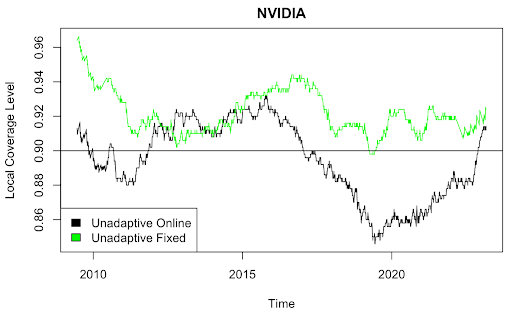
\includegraphics[width=0.5\textwidth,height=\textheight]{./images/3nvidiaqs.png}
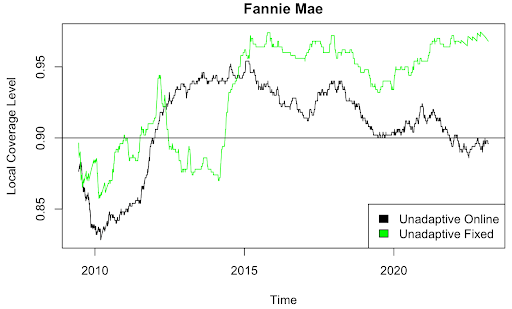
\includegraphics[width=0.5\textwidth,height=\textheight]{./images/4fmqs.png}

Moving to ACI, varying-\(QS\) (``original method'') performs similarly
to fixed-\(QS\) (``fixed method'') for the NVIDIA dataset, but shows
significantly more variability in local coverage for Fannie Mae. This is
related to the fact that Fannie Mae's fixed-\(QS\) \(\alpha_t\) is much
more variable than its varying-\(QS\) \(\alpha_t\). An interesting
situation arises for Fannie Mae post-2015: \(\alpha_t\) is significantly
elevated in the fixed-\(QS\) method, but local coverage is similar for
both methods. Both of these observations again point to the fact that
varying \(Q\) and \(S\) dampen the need for variation in \(\alpha_t\),
allowing \(\alpha_t\) to remain near \(\alpha\) over time with variation
to help account for rapid shifts.

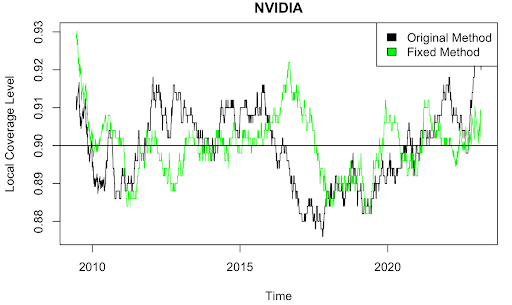
\includegraphics[width=0.5\textwidth,height=\textheight]{./images/5nvidia2qs.png}
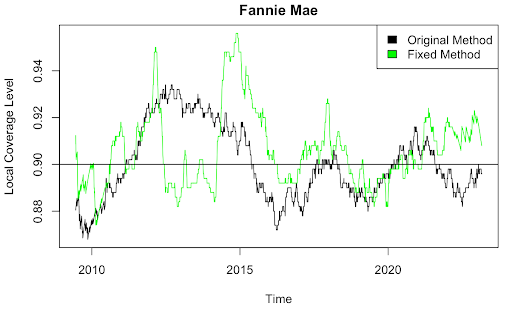
\includegraphics[width=0.5\textwidth,height=\textheight]{./images/6fm2qs.png}
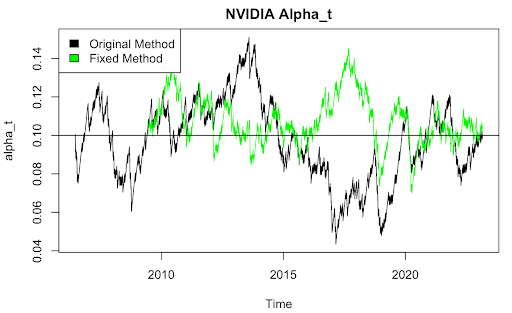
\includegraphics[width=0.5\textwidth,height=\textheight]{./images/7nvidia3qs.png}
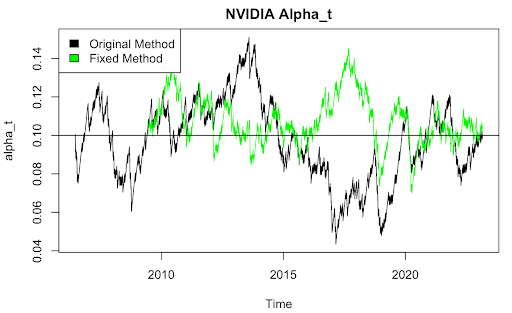
\includegraphics[width=0.5\textwidth,height=\textheight]{./images/8fm3qs.png}

Of course, this experiment's external validity is very limited: it's
possible that differences we observe are unique to these datasets.
Still, these results do support the intuition that the performance
guarantee for ACI under fixed-\(QS\) would hold under varying-\(QS\). On
the other hand, they don't provide any strong evidence for better
performance. One hypothesis emerging from this experiment is that the
local performance guarantee proof's setting (a smaller distribution
shift with fixed-\(QS\)) may be equivalent to a
larger-distribution-shift setting with varying-\(QS\) for the purposes
of the proof, since retraining \(Q\) and \(S\) dampens the effective
distribution shift faced by \(\alpha_t\).

\hypertarget{possible-other-extensions}{%
\section{Possible Other Extensions}\label{possible-other-extensions}}

We mention here but do not implement a number of other possible
extensions to the paper:

\begin{itemize}
\tightlist
\item
  It would be useful to experiment, possibly via simulation, with the
  method's performance under different forms of nonstationarity. Similar
  to the fixed-\(QS\) analysis above, this could provide support for or
  against the broader applicability of the local performance guarantee.
\item
  The weighted method proposed by the authors could be better analyzed,
  both theoretically and over a broad range of weights (extending to
  uniform weights). The authors say that they found it to be similar in
  performance to the unweighted method, but only mention testing it with
  a quite rapid decrease in weight going back in time.
\item
  On a related note, it would be valuable to evaluate other methods of
  adding momentum to \(\alpha_t\) updates. For example, if we have
  missed coverage quite a few times recently, we guess that we are in
  the midst of a distribution shift and so accelerate quantile widening
  by even more. Specifically, we could apply momentum implementations
  similar to those often used in gradient descent. This would make sense
  in light of the online-learning view of the \(\alpha_t\) updates
  (although, unlike in many other gradient-descent settings,
  \(\alpha_t\) optimization must be convex). The weighting proposed by
  the authors achieves this to a significant degree (in fact, they call
  the weighting ``momentum'' in their code!) but is not directly
  equivalent to several other momentum approaches.
\item
  The authors apply ACI to prediction of the next time step, but it
  could be extended in a straightforward manner to prediction intervals
  for longer forecast horizons, which would be updated each time step as
  well.
\item
  Finally, it would be interesting to explore the use of ACI in a
  setting where the prediction model is moving between different
  environments (as opposed to the environment changing over time).
\end{itemize}

\hypertarget{conclusion}{%
\section{Conclusion}\label{conclusion}}

As proposed by Gibbs and Candès, adaptive conformal inference is a
powerful extension of conformal inference for the online setting;
despite some limitations in its performance guarantees, it appears to
perform quite well in practice. ACI provides a solid platform for
additional experimentation and extension.

\hypertarget{code-additional-figures}{%
\section{Code \& Additional Figures}\label{code-additional-figures}}

\url{https://github.com/ajkeller10/multiple-testing-final-project}

\end{document}
